 \newcommand{\atom}{atom\xspace}
 \newcommand{\atoms}{atoms\xspace}  
 \newcommand{\pushSymbol}{{\vartriangleright}}
\newcommand{\Push}[4] {\ensuremath{(\overline{#1 \mapsto #2}, #3) \pushSymbol #4}}
\newcommand{\Pushes}[2] {\ensuremath{(\overline{#1}) \pushSymbol #2}}
\newcommand{\va}{\ensuremath{\upsilon}}

 
\section{\LangOO -- a small  object oriented programming language}

\subsection{\LangOO syntax runtime configurations}
\label{sub:Loo} 
 \LangOO  is a {small}, imperative, sequential,  class based, typed, object-oriented language, whosefields are private to the class where they are defined -- similar to the one in OOPSLA\footnote{any differences?}.
The complete definition of \LangOO  {can be found in the appendices  \cite{necessityFull}.}
A \LangOO state $\sigma$ consists of a  heap $\chi$, and a  {stack $\psi$ which is a sequence of frames}.
A frame, $\phi$, consists of local variable map, and a continuation, \ie a sequence of statements to be executed.
 
Modules are mappings from class names to class definitions. 
Execution takes place in the context of  a module $M$ and   a state $\sigma$, defined via unsurprising small-step semantics of the form \ \ 
   $M, \sigma \leadsto \sigma'$. \ \
The   top frame's continuation contains the statement to be  executed next.  



\sdN{
\paragraph{Notation and Naming conventions} We adopt the following, un-surprising, notation:
% OOPSLA, where
\begin{itemize}
\item
$\alpha$, $\alpha'$, $\alpha_1$, ... are addresses,   $x$, $x'$, $x_1$, ..., $y$, ... $z$, ... are variables, and $\va$, $\va'$ ... are either addresses or variables, we call these \emph{\atoms}.
\item
Simple expression, $e$, are defined in Def. \ref{def:assert:syntax}. They are simple expressions, which may contain variables, addresses, field look-ups, as well as ghost-field look-ups, but \emph{not} method calls.
\item
$\alpha \in \sigma$ means that $\alpha$ is defined in the heap of $\sigma$, and $x\in \sigma$ means that $x$ is defined in the top frame of $\sigma$. Conversely, $\alpha$ is fresh, resp.$x$ is fresh in $\sigma$   in $\sigma$ means that $\alpha\notin\sigma$, resp. $x\notin\sigma$, and $x$ is fresh in assertion $A$ means that $x$ does not appear free in $A$.
\item
$\interpret{\sigma}{\alpha}$  is $\alpha$; and $\interpret{\sigma}{x}$  is the value to which  $x$  is mapped in the top-most frame of $\sigma$'s stack; 
and $\interpret{\sigma}{e.f}$ looks up in $\sigma$'s heap the value of $f$ for the object  $\interpret{\sigma}{e}$.
Note that $\interpret{\sigma}{e}$ is not defined when $e$ contains a method call ot a ghost field.
\item The substitution  $\sigma[x \mapsto \alpha]$ is applied to the top frame of $\sigma$, and $\sigma[\overline{x \mapsto \alpha}]$ applies the substitutions $\overline{x \mapsto \alpha}$ to the top frame.
\item The substitution $A[\sigma]$ replaces in $A$ all its free variables, $\overline x$, by their values,  $\overline{\interpret{\sigma}{x}}$.
\item 
$\Push{z}{\alpha}{s}{\sigma}$ pushes onto the stack of $\sigma$ a new frame, with local variable mapping $\overline {z}$ onto $\overline {\alpha}$ and  continuation $s$,  and leaves the heap unmodified. It corresponds to the first step of a  method call, and is defined only if $z_0$ is \prg{this}, and   $\overline {z}$ has the same cardinality as  $\overline {\alpha}$. The set 
$ \Pushes {\alpha} {\sigma}$ is the set of states, $\sigma'$ such that  $\sigma'=\Push{z}{\alpha}{s}{\sigma}$ for some $\overline z$ and some $s$.
\item
$C\in M$ means that class $C$ is in the domain of module $M$. 
% perhaps we do not need to expose the below
% The terms $\sigma.\prg{stack}$,   $\sigma.\prg{contn}$,  $\sigma.\prg{heap}$     mean the stack, the continuation at the
%top frame of $\sigma$, %resp. 
% and the heap of $\sigma$.
% The term $\alpha\!\in\!\sigma.\prg{heap}$ means that $\alpha$ is in the domain of the heap of $\sigma$, and \emph{$x$ fresh in $\sigma$} means that 
\end{itemize}
}

\paragraph{Applicability} 
While our work is based on a simple, imperative, typed, object oriented  language with unforgeable addresses and private fields, we believe that % our approach
 it is applicable to several programming paradigms, and  that   unforgeability and privacy
 can be replaced  by lower level mechanisms such as capability machines \cite{vanproving,davis2019cheriabi}.
  
\subsection{Execution and Bounded Execution}
 
In appendix ??? we  define execution  of \Loo\footnote{check whether it is Tool, or Loo, or what};
 it is a small steps operational semantics of the shape $\leadstoOrig  {M} {\sigma_1}   {\sigma_2}$. 
 The relation $\leadstoOrigStar  {M} {\_}   {\_}$  is the reflexive, transitive closure of $\leadstoOrig  {M} {\_}   {\_}$ .
The semantics is un-surprising. 
 A statement may assign to variables, allocate a new object, 
perform field reads and writes on objects,  or
 call methods on those objects. 
In particular, the code to be executed by a method call is kept in a continuation within the frame for that call. When a method is called, a new frame is pushed on to the stack; this frame  maps \prg{this} and the formal parameters to  the values for the receiver and other arguments, and the continuation to the body of the method.  When the continuation is final\footnote{TODO check and define}, the frame is popped and the value from the last frame's continuation is entered into the caller's continuation. 
%In other aspects, the semantics is un-surprisring.%we return from that call, its frame is  popped, and execution continues in the context of the calling method.

%\sdN{
%  \begin{definition}[Execution]
%\label{def:deep}
%The relation  $\leadstoOrig  {M} {\sigma_1}   {\sigma_2}$ is defined  in appendix ... The relation $\leadstoOrigStar  {M} {\_}   {\_}$  is the reflexive, transitive closure of $\leadstoOrig  {M} {\_}   {\_}$ .
%\end{definition}
%}

\sdN{Fig. \ref{fig:UpSemantics} demonstrates  such  execution steps:  black disks indicate states;
 horizontal $\leadsto$-arrows denote   steps  within the same  call; upwards arrows denote  method calls;
 %(pushing a new frame onto the stack);  
 downwards arrows denote method returns. % (popping the top of the stack). 
 Here,   $\leadstoOrig M {\sigma_8}   {\sigma_9} $ is a step within the same call, $\leadstoOrig M {\sigma_9}   {\sigma_{10}} $ is a method call  %(say a call to $m_a$), 
with $\leadstoOrig M {\sigma_{12}}   {\sigma_{13}} $ %is a method return  (from the call to $m_a$), 
the corresponding return. %, while  $\leadstoOrig M {\sigma_{16}}   {\sigma_{17}} $ is another  method call  %(say a call to $m_b$),  and 
%with $\leadstoOrig M {\sigma_{18}}   {\sigma_{19} }$ the corresponding return.
}
%is another  method call  (from the call to $m_b$).}
% for example  we depict a case where we are executing a method (say $m_a$), which eventually calls another method (say $m_b$), and which in tis turn calls a further method (say $m_c$): We start at $\sigma_1$ and in one step we reach $\sigma_2$, which is a method  call  to $m_b$. 
%This leads to state $\sigma_3$, and after another step we reach $\sigma_5$, which is a method call to $m_c$, 
%leading to state $\sigma_5$ and $\sigma_6$. 
%The latter is the return, leading to $\sigma_7$, which again, is a return, leading to $\sigma_8$.}

\begin{figure}[htb]
\begin{tabular}{|c|}
 \hline %  \\ -- this added one vertical space
\resizebox{6cm}{!}{
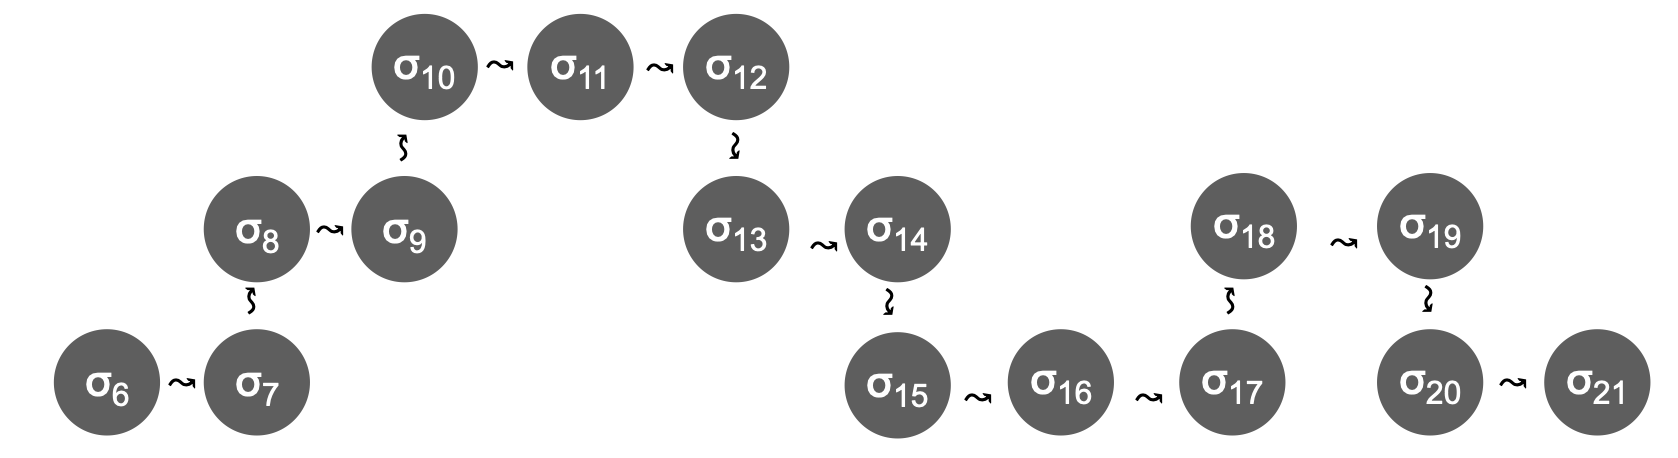
\includegraphics[width=\linewidth]{diagrams/bounded.png}
} 
 \\
\hline
\begin{tabular}{l|l}
\ \ \ \ \ \ \  \ \ \ \ \ \ \  \ \ \ \ \ Execution \ \ \ \  &  \ \ \ \ \ \ \  \ \ \ \ \ \ \   \ \ \ \ \  Bounded Execution \ \ \ \  \\
\hline % \\
 $\leadstoOrig  M  {\sigma_8}    {\sigma_9} $ \ \ \ \ \ \ \ \  \ $\leadstoOrig  M  {\sigma_9}    {\sigma_{10}} $ & 
%Bound
\ \ \  $\leadstoBounded  M  {\sigma_8} {\sigma_8}  {\sigma_9} $ \ \ \ \ \ \ \ \  \ $\leadstoBounded  M  {\sigma_9} {\sigma_8}  {\sigma_{10}} $
\\
$\leadstoOrig  M  {\sigma_{12}}   {\sigma_{13}} $ \ \ \ \ \ \ \  $\leadstoOrig  M  {\sigma_{13}}    {\sigma_{14}} $  & 
%Bound
\ \ \  $\leadstoBounded  M  {\sigma_{12}} {\sigma_8}  {\sigma_{13}} $ \ \ \ \ \ \ \  $\leadstoBounded  M  {\sigma_{13}}  {\sigma_{8}}  {\sigma_{14}} $ 
\\ 
%ORIG
$\leadstoOrig M {\sigma_{14}}   {\sigma_{15}} $  \ \ \ \ \ \ \  
\ \ \ \ \ \ \  \ \ \ & \ \ \ 
%BOUND
$\notLeadstoBounded  M  {\sigma_{14}} {\sigma_8}  {\sigma_{15}} $
\end{tabular}
\\
\hline
\end{tabular}
   \caption{Ilustrating
    Def. \ref{def:deep}  and \ref{def:shallow:term})%
    }
   \label{fig:UpSemantics}
 \end{figure}
 
\sdN{Note that $\leadstoOrig M {\sigma_{8}}   {\sigma_{9}} $ and $\leadstoOrig M {\sigma_{13}}   {\sigma_{14}} $ are steps within the same call, but 
$\leadstoOrig M {\sigma_{14}}   {\sigma_{15}} $ and $\leadstoOrig M {\sigma_{17}}   {\sigma_{18}} $ are not. %steps within the same call,
% even though all four states ($\sigma_{13}$, $\sigma_{14}$, $\sigma_{17}$, and $\sigma_{18}$), have the same number of frames on their stack.
We want a semantics to reflect whether execution steps happen within the bounds of certain call. For this, we define \emph{bounded execution}, 
$\leadstoBounded {M} {\sigma} {\sigma''} {\sigma'}$ 
which are execution steps which lead from $\sigma$ to $\sigma'$ while not popping  $\sigma''$-s top frame.
Formally,
}

{
\begin{definition}[Bounded Executions]
\label{def:shallow:term}
We define the relation  $\leadstoBounded {M} {\sigma_1} {\sigma} {\sigma_2}$ 

\begin{itemize}
\item
 $\leadstoBounded {M} {\sigma_1} {\sigma} {\sigma_2}$ \ \ \ iff \ \ \  $\leadstoOrig {M} {\sigma_1} {\sigma_2}$\\
$\strut  \hspace{3.6cm} \wedge $\\
$\strut  \hspace{3.1cm}\ \    \exists \phi,\psi, \phi_1, \phi2.[ \ \sigma = (\phi\cdot\psi,\_) \ \wedge \ \sigma_1 = (\psi_1\cdot \psi, \_)
\ \wedge\ \sigma_2 = (\psi_2\cdot \psi, \_)\ ] $ 
\item
 $\leadstoBoundedStar {M} {\_} {\sigma} {\_}$\ \  is the reflexive, transitive closure of $\leadstoBounded {M} {\_} {\sigma} {\_}$.
\end{itemize}
\end{definition}
}
 
 \sdN{Continuing our discussion of Fig. \ref{fig:UpSemantics}, notice that $\leadstoOrig {M} {\sigma_{14}}  {\sigma_{15}}$ 
 but    $\notLeadstoBounded  {M}  {\sigma_{14}} {\sigma_8} {\sigma_{15}}$:  this step would pop  $\sigma_8$'s
 top frame. 
Therefore, 
 $\leadstoOrigStar {M} {\sigma_8}  {\sigma_{15}}$ 
 but  $\notLeadstoBoundedStar {M} {\sigma_8} {\sigma_8} {\sigma_{15}}$, and also
  $\leadstoOrigStar {M} {\sigma_8}  {\sigma_{18}}$ 
 but  $\notLeadstoBoundedStar {M} {\sigma_8} {\sigma_8} {\sigma_{18}}$  -- the latter reflects that $\sigma_8$ and $\sigma_{18}$ belong to different calls. 
}

  \subsection{{Reachable  Objects}}
  
{The  \SpecLang  specifications support universal quantification over  objects; such specifications 
are applicable  to all objects in the heap witch, are however, either locally reachable (i.e. there is in the heap a path from the an 
object on the top frame to the particular object), or globally reachable (i.e. there is in the heap a path from the an 
object on some frame to the particular object.)
In this section  we will formally define these concepts.}\footnote{TODO we need a better motivation for these concepts.}
 



We define  locally reachable, $ \LRelevant \alpha \sigma $, as  the objects  $\alpha$ which are reachable the top frame on the stack of $\sigma$,
and globally reachable, $\GRelevant \alpha \sigma$, as the objects  $\alpha$ which  are reachable from any  frame on the stack of $\sigma$.
 
\begin{definition} We define 
\begin{itemize}
\item
$ \LRelevant \alpha \sigma $ \ \ iff\ \  
$\exists \phi.[\ \sigma=(\phi\cdot\_, \_)$ and $\Relevant \alpha \phi \sigma\ ]$. % for some $\phi$
\item
$\GRelevant \alpha \sigma$  \ \ iff\ \  
$\exists \phi.[\ \sigma=(\_\cdot\phi\cdot\_, \_)$ and $\Relevant \alpha \phi \sigma\ ]$. % for some $\phi$
\end{itemize}
where\\
$\strut\ \ \ \  \ \ \ \ \ \ \Relevant \alpha \phi \sigma $  \ \ \ \ \ \ \ iff\ \  
$\exists n\in \mathbb{N}.\exists \prg{f}_1,... \prg{f}_n.\exists \prg{x}.[ \ \interpret{\sigma}{\phi(x).\prg{f}_1.....\prg{f}_n} = \alpha \ \ ]$.

\end{definition}


The lemma below says that (1) Any locally reachable object is globally reachable, and 
(2) Any object which existed in the current  heap, and is globally reachable at some future point is globally reachable now: that is, 
no globally unreachable object may become reachable.\footnote{cite "only connectivity begets connectivity"}, and
\sdN{(3) the objects locally reachable after a method call were also locally reachable before the call; the requirement in
the premise  that the arguments of the call, $\overline o$, are locally reachable is not a restriction, because, by construction, the arguments to a method call are locally reachable.}



\begin{lemma}
\label{lemma:relevant}
For all modules $M$, states $\sigma$, $\sigma'$, for all objects $o$, ${\overline o}:$\footnote{\sdN{TODO decide whether $o$ or $\alpha$}}
%and  variables ${\overline z}$, and statements $s:$
\begin{enumerate}
\item
$ \LRelevant \alpha \sigma\ \ \Longrightarrow \ \   \GRelevant \alpha \sigma$
\item
$M, \sigma  \leadsto^*   {\sigma'} \ \wedge \  \GRelevant o {\sigma'} \ \wedge \ o\in dom(\sigma) \ \ \Longrightarrow \ \  \GRelevant o {\sigma}$
\item
\sdN{$\LRelevant {\overline o} {\sigma} \ \ \wedge \sigma'\in \Pushes{o} {\sigma}\ \ \wedge \  \LRelevant o {\sigma'} \ \ \ \Longrightarrow \ \ \  \LRelevant o {\sigma}$
}
\end{enumerate}
\end{lemma}

 
 \begin{figure}[htb]
\begin{tabular}{|c|c|c|}
\hline \\
\resizebox{3.5cm}{!}{
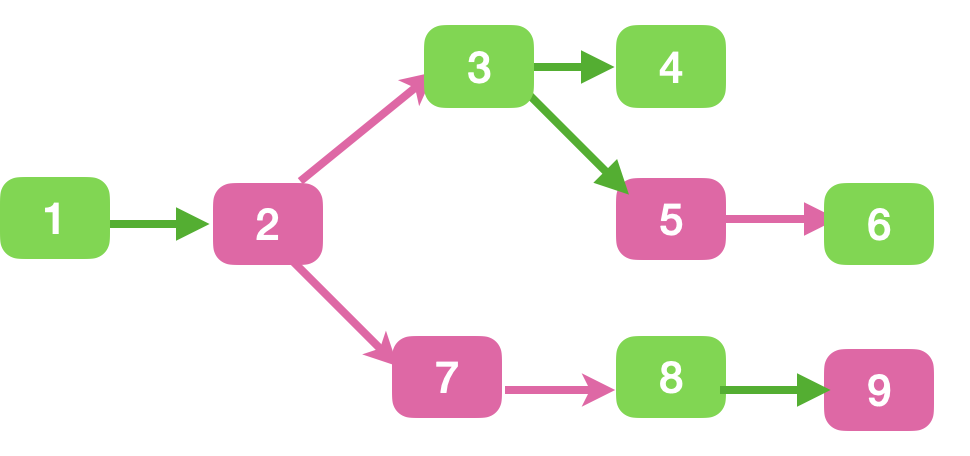
\includegraphics[width=\linewidth]{diagrams/heap.png}
} 
&
\resizebox{5cm}{!}{
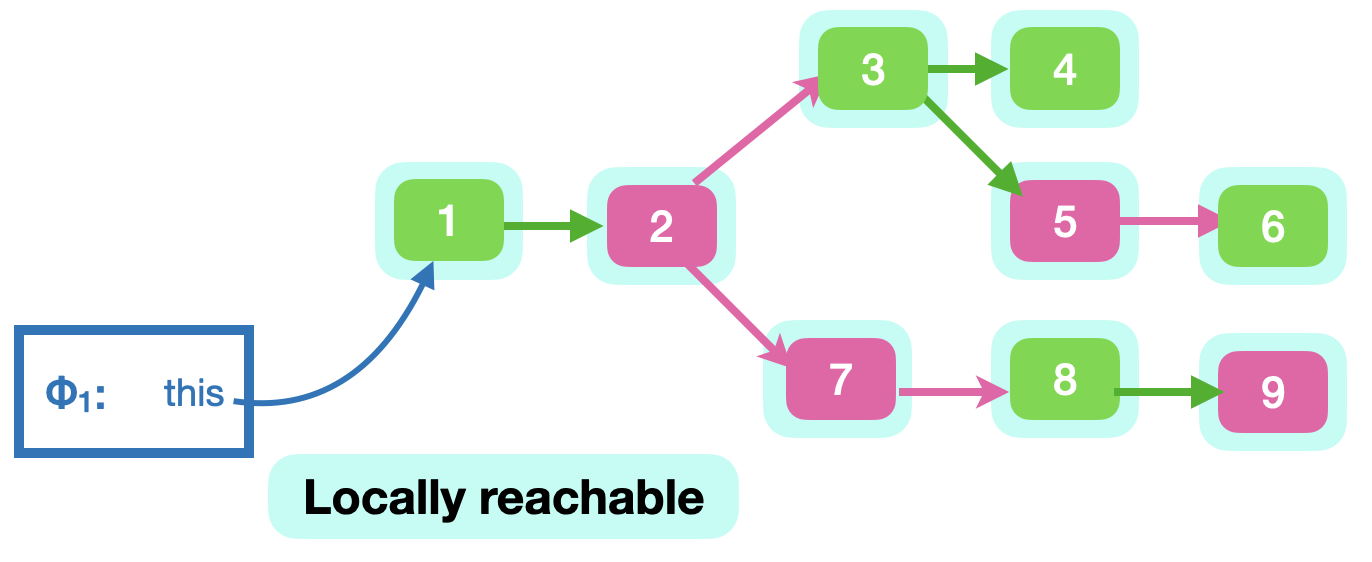
\includegraphics[width=\linewidth]{diagrams/locReachA.png}
} 
&
\resizebox{5cm}{!}{
\includegraphics[width=\linewidth]{diagrams//locReachb.png}
} 
\\
\hline
 a heap
&
Locally Reachable from $\phi_1$
&
Locally Reachable from $\phi_2$
\\
\hline \hline
\end{tabular}
   \caption{A heap, and locally Reachable Objects from $\phi_1$ and $\phi_2$ }
   \label{fig:LReachable}
 \end{figure}

   
\subsubsection{{Reachable  Objects and Bounded Execution}}


The lemma below is the counterpart to lemma \ref{lemma:relevant} --  with the difference that  \ref{lemma:relevant:after:bounded} has the  stronger  premise  , as it requires bounded executions. 

\begin{lemma}
\label{lemma:relevant:after:bounded}
For all states $\sigma$, $\sigma'$, and $\sigma''$,for all objects $o$, and for all modules  $M$:
\begin{itemize}
\item
${\leadstoBoundedStar {M}  {\sigma} {\sigma''} {\sigma'}} \ \ \wedge \ \  \GRelevant o {\sigma'} \ \ \wedge\ \ o\in dom(\sigma)\ \ \ \Longrightarrow \ \  \ \GRelevant o {\sigma}$.
\item
${\leadstoBoundedStar {M}  {\sigma}  {\sigma} {\sigma'}} \ \ \wedge \ \   \LRelevant o {\sigma'}\  \ \wedge\ \ o\in dom(\sigma)\ \ \ \Longrightarrow \ \ \ \LRelevant o {\sigma}$.
\end{itemize}
\end{lemma}

\sdN{Consider Fig.  \ref{fig:UpSemantics}, the lemma above promises that any objects locally reachable in $\sigma_{14}$ which already existed in $\sigma_{8}$, were locally accessible in $\sigma_{8}$. However, the lemma is only  applicable to bounded execution, and as 
$\notLeadstoBoundedStar {M} {\sigma_8} {\sigma_8} {\sigma_{17}}$, 
the lemma does not promise that  objects locally reachable in $\sigma_{17}$ which already existed in $\sigma_{8}$, were locally accessible in $\sigma_{8}$ -- namely it could be hat object are made globally reachable during the step from $\sigma_{15}$ to $\sigma_{16}$.}








